\documentclass[12pt]{article}
\usepackage{fontspec}

\setmainfont{Times New Roman} % Times New Roman, Arial, Calibri

\usepackage{setspace}
\setstretch{1.15}

\usepackage{pdflscape}

\usepackage{graphicx}
\usepackage{float}
\usepackage{placeins}
\usepackage[backend=biber, style=numeric, sorting=none]{biblatex}
\addbibresource{references.bib}

\usepackage{geometry}
\geometry{top=2.5cm, bottom=2.5cm, left=2.5cm, right=2.5cm}

\usepackage{pdfpages}

\usepackage{listings}
\usepackage{xcolor}
% Define colors
\definecolor{codegreen}{rgb}{0,0.6,0}
\definecolor{codegray}{rgb}{0.5,0.5,0.5}
\definecolor{codepurple}{rgb}{0.58,0,0.82}
\definecolor{backcolour}{rgb}{0.95,0.95,0.92}

% Setup the listings package
\lstdefinestyle{mystyle}{
    backgroundcolor=\color{backcolour},
    commentstyle=\color{codegreen},
    keywordstyle=\color{magenta},
    numberstyle=\tiny\color{codegray},
    stringstyle=\color{codepurple},
    basicstyle=\ttfamily\footnotesize,
    breakatwhitespace=false,
    breaklines=true,
    captionpos=b,
    keepspaces=true,
    numbers=left,
    numbersep=5pt,
    showspaces=false,
    showstringspaces=false,
    showtabs=false,
    tabsize=2
}

\lstset{style=mystyle}

\usepackage{amsmath} % For mathematical features

\renewcommand{\theequation}{\thesection.\arabic{equation}}
\renewcommand{\thefigure}{\thesection.\arabic{figure}}

\usepackage{chngcntr}
\usepackage{amssymb}
\counterwithin{figure}{section}
\counterwithin{equation}{section}

\title{Identifying Dynamic Systems with Probabilistic Numerics}
\author{Harvey Walton}
\date{\today}

%Repeated Text
\newcommand{\ndiFigCaption}[1]{The rectangle method for finding the #1 bound of the integral of the standard Gaussian (normal) distribution between -2 and 1.}

\hyphenpenalty=700
\exhyphenpenalty=700

\begin{document}
    \pagenumbering{roman}

    \thispagestyle{empty}
    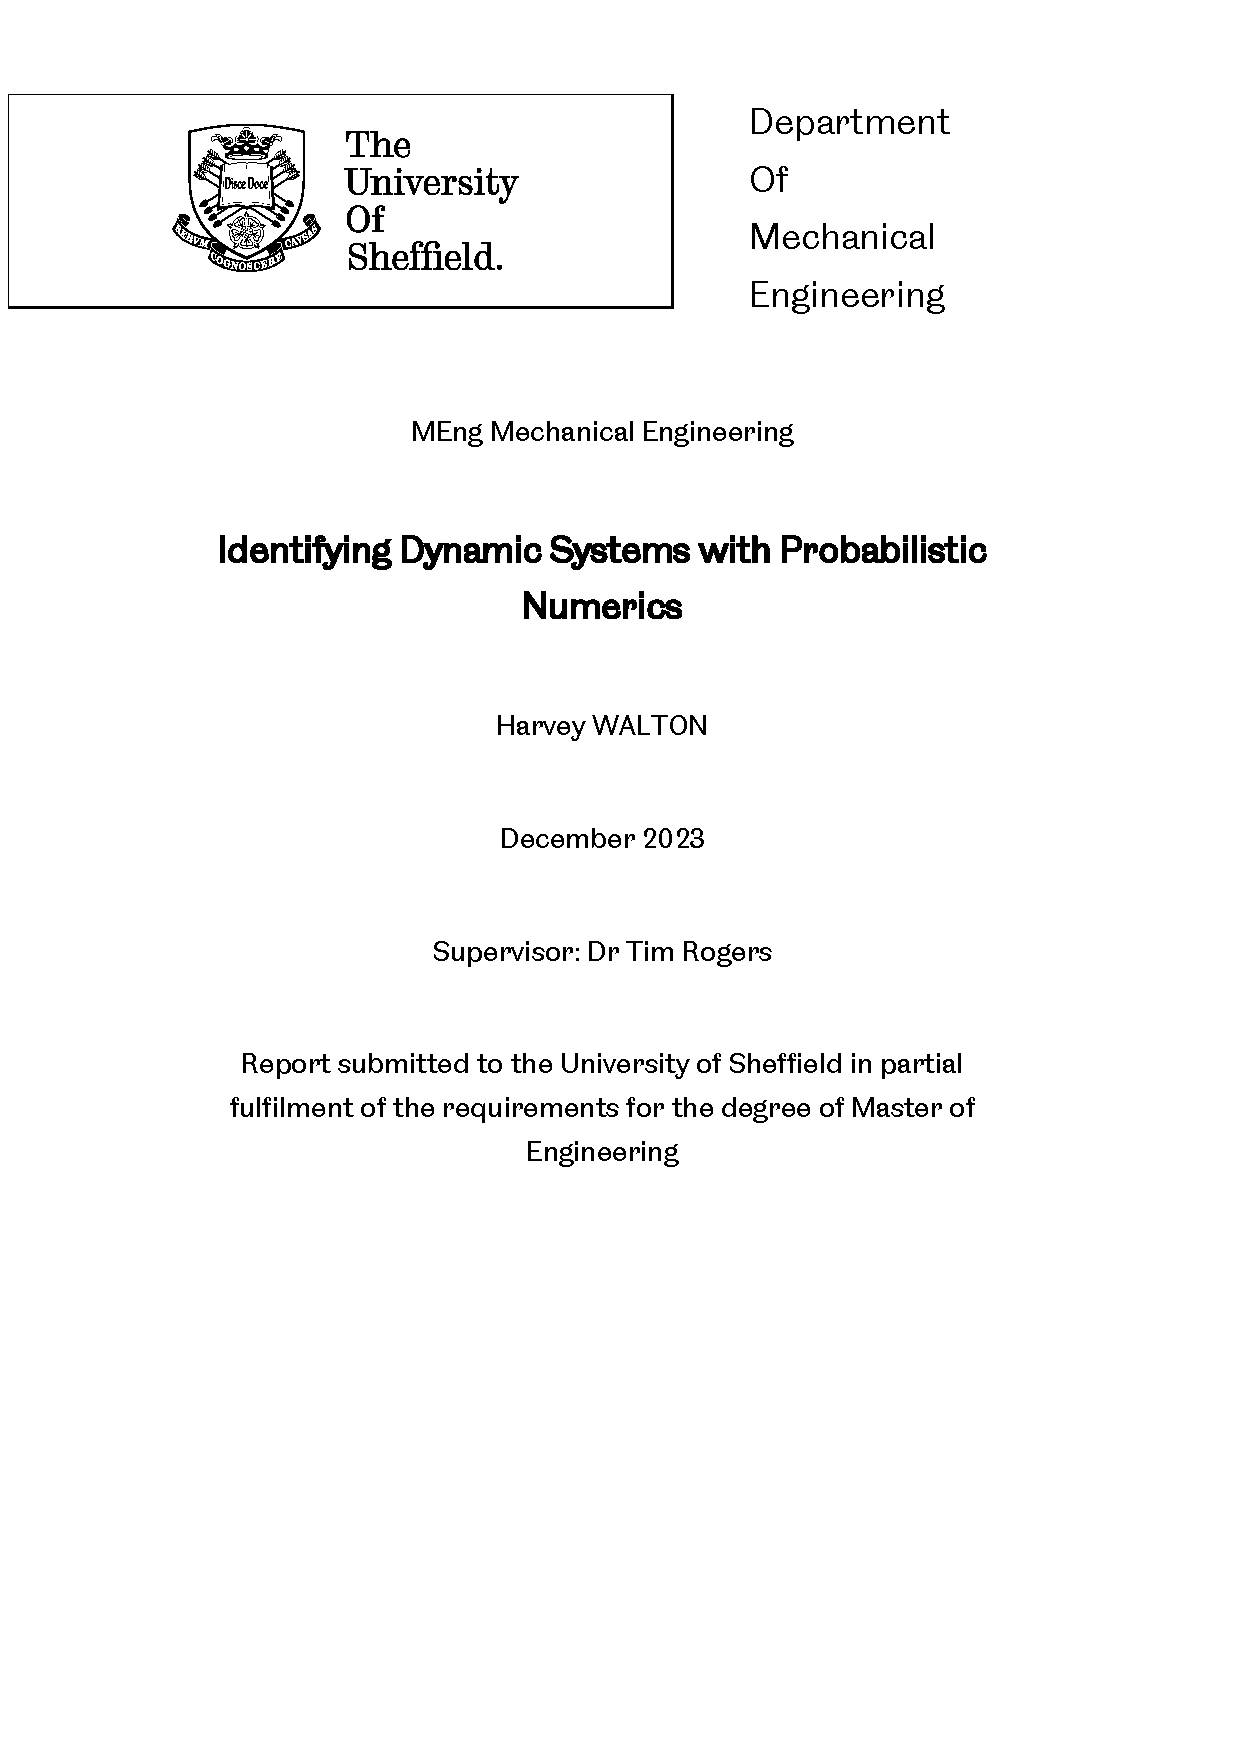
\includepdf[pages=1, frame, scale=1.09, pagecommand={}, offset=0 -35]{figures/titlepage.pdf}

    \section*{Nomenclature}
    \begin{tabular}{ll}
        $p(x)$ & Probability density function of arbitrary variable, $x$ \\
        $\sigma$ & Standard deviation \\
        $\sigma^2$ & Variance hyperparameter in the context of a kernel \\
        $\mu$ & Mean value \\
        $\pi$ & Mathematical constant, Pi \\
        $h$ & Incremental distance used in gradient calculation \\
        $f(x)$ & Latent function of the variable $x$ \\
        $f^*$ & An array of values of the Latent function evaluated at a set of test points \\
        $y_n$ & Noisy observed output based on the latent function, $f(x)$\\
        $y$ & An array of $y_n$ values from a set of training points \\
        $\epsilon_n$ & Noise in observation, normally distributed \\
        $\mathcal{N}$ & Normal (Gaussian) distribution \\
        $K$ & Covariance matrix of the Kernel function, k \\
        $K_{X,X}$ & Covariance matrix for training input data, $K(X,X)$ \\
        $K_{X,*}$ & Covariance matrix between training inputs and test inputs, $K(X,X_*)$ \\
        $K_{*,*}$ & Covariance matrix for test inputs, $K(X_*,X_*)$ \\
        $I$ & Identity matrix \\
        $\sigma^2_y$ & Variance of observation noise \\
        $\theta$ & Set of hyperparameters \\
        $D$ & Training data \\
        $N$ & Number of data points \\
        $K_{\sigma}$ & Covariance matrix with noise term, $K_{X,X} + \sigma^2_y I$ \\
        $\mu_{*|X}$ & Conditional mean of the Gaussian Process, given the training data X \\
        $\Sigma_{*|X}$ & Conditional covariance of the Gaussian Process, given the training data X \\
        $\omega$ & Angular frequency \\
        $F(\omega)$ & Fourier transform of $f(t)$ \\
        $i$ & Imaginary unit \\
        $K_{ij}$ & Element of a covariance matrix \\
        $\mathbf{x}_i, \mathbf{x}_j$ & Input vectors \\
        $\sigma$ & Standard deviation \\
        $k(x, x')$ & Kernel function of arbitrary points, $x$, and $x'$ \\
        $p$ & Period hyperparameter in periodic kernel \\
        $l$ & Length hyperparameter in periodic kernel \\
        $m$ & Number of inducing points in Sparse GP \\
        $\text{MSE}$ & Mean Squared Error \\
        $A_i$ & Value of arbitrary function, A, at index i  \\
        $B_i$ & Value of arbitrary function, B, at index i \\
    \end{tabular}


    \newpage
    \tableofcontents
    \newpage

    \pagenumbering{arabic}

    \section{Background and Understanding of the Problem}


    Problems in engineering are typically described initially using a framework of continuous mathematical functions.
    This means that their output has no jumps or gaps in values, and they can be evaluated using input values that are on a sliding scale of a continuous input domain.
    For example, time in the real world is on a continuous sliding scale, which means that any interval in time can always be subdivided into a smaller interval.
    Continuous functions in turn can often be manipulated analytically using mathematical transformations.
    For example, if the velocity of a particle is given as a continuous function of time, a continuous acceleration function can be derived from the velocity analytically through a mathematical process called differentiation.

    \subsection{The Limits of the analytical approach}

    However, there are many situations where this analytical approach is unsuitable.
    Classically, numerical methods will be used to approximate the true solution to the transformation.

    \subsubsection{Intractable Complexity}\label{subsubsec:int-comp}

    The first reason for this is that the analytical approach may be too complex for anyone to solve.
    A good example of this is the Gaussian (normal) distribution (Equation~\ref{eq:norm}). %\cite{NIST2023}

    \begin{equation}
        p(x) = \frac{1}{\sigma\sqrt{2\pi}} \exp\left(-\frac{(x - \mu)^2}{2\sigma^2}\right)\label{eq:norm}
    \end{equation}

    This is a common continuous probability distribution characterized by a bell-shaped curve, and is defined its mean ($\mu$) and variance ($\sigma^2$). The mean determines the centre of the distribution and the variance measures the spread.
    The definite integral of this is often needed in order to find cumulative probabilities (i.e., the chances of a continuous random variable being in a range defined by two values).
    This process can be visualised as finding the area underneath the curve between 2 input values (Figure~\ref{fig:ndi_}).

    \begin{figure}[htbp]
        \centering
        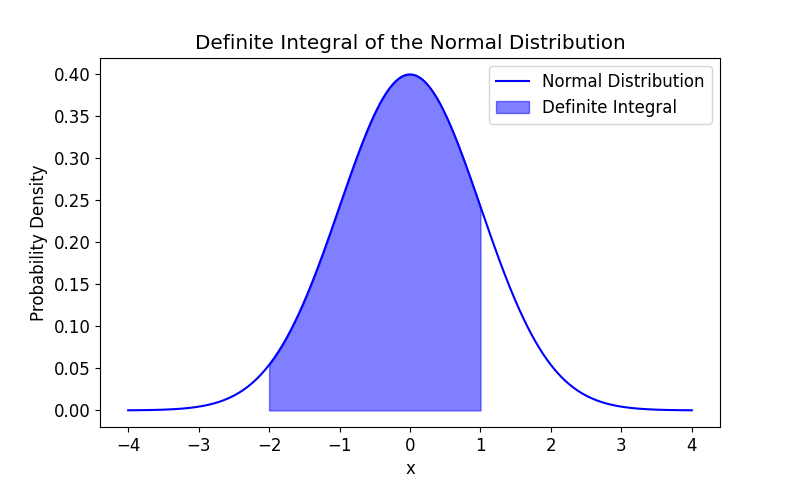
\includegraphics[width=0.8\linewidth]{figures/ndi/ndi_}
        \caption{A definite integral between -2 and 1 of the standard Gaussian (normal) distribution. This is used to find cululative probabilities.}
        \label{fig:ndi_}
    \end{figure}

    In this case, a numerical method is typically used instead such as the Rectangle Method, which uses the Riemann integral definition.
    This states that an integral can be approximated by summing the area of many adjacent rectangles between the function and the axis~\cite{NumericalAnalysis2023}, as shown in Figure~\ref{fig:ndi-num_} and Figure~\ref{fig:ndi-num2_}.

    \FloatBarrier

    \begin{figure}[htbp]
        \centering
        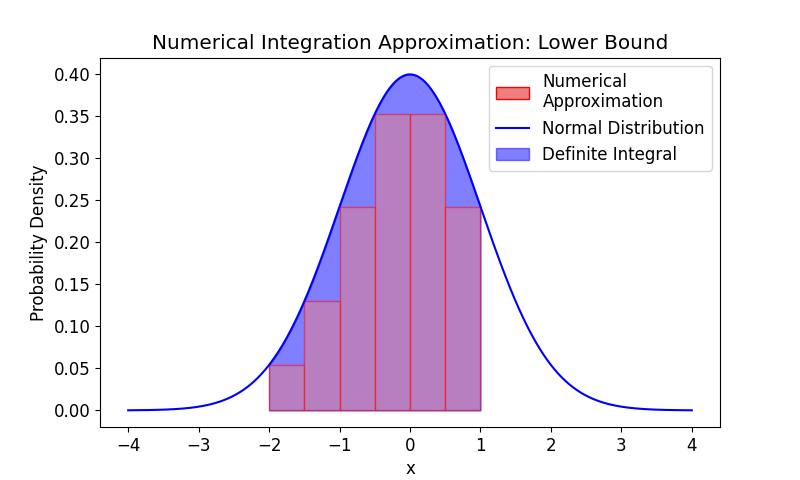
\includegraphics[width=0.8\linewidth]{figures/ndi-num/ndi-num_}
        \caption{\ndiFigCaption{lower}}
        \label{fig:ndi-num_}
    \end{figure}

    \FloatBarrier

    \begin{figure}[htbp]
        \centering
        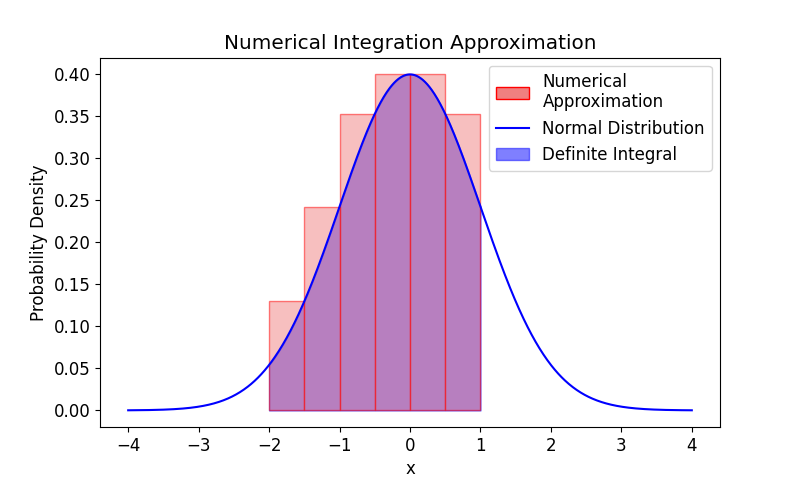
\includegraphics[width=0.8\linewidth]{figures/ndi-num2/ndi-num2_}
        \caption{\ndiFigCaption{upper}}
        \label{fig:ndi-num2_}
    \end{figure}

    As you can see, there are two ways to draw the rectangles.
    In the first method, the top corner of the two that touches the curve is chosen such that the top edge is below the curve.
    This provides an underestimate, which we can use as a lower bound to the true value of the integral.
    Whereas in the second method, the top corner of the two that touches the curve is chosen such that the top edge is above the curve.
    This provides an overestimate, which we can use as an upper bound to the true value of the integral.
    Classically, the quality of this numerical methods are computed using the ``error bounds'' ie range between these upper and lower values.
    As the width of the rectangles approaches zero, the approximation increasingly converges to the exact value of the integral.
    This can never happen in practice, however, because it would require infinite computational work, but we can get precise approximations with small error bounds none-the-less.

    \subsubsection{Data Sampling}
    The second situation where the analytical approach is unsuitable is when working with real world data.
    Here, the real world continuous data streams of the variables you are measuring must be sampled at a number of individual (or ``discrete'') points in time.
    A simple example of this is how a video camera discretises the continuous events of the world into individual frames (or ``samples'') that can be replayed back-to-back to recreate an approximation of the events.
    As the frame rate increases, the events are represented more faithfully, but the amount of information required to store the approximation tends to infinity as the length of time between frames tends to zero, which is not possible in practice.
    This discrete data is unsuitable for performing transformations analytically because they rely on the data being continuous.
    Again, there are numerical methods that are commonly used to approximate this instead.

    For example, differentiation is the process of finding the gradient of a continuous function at any location along the curve.
    For a discrete function, the gradient at any point is undefined because you cannot have a tangent of a point.
    However, it is possible to approximate the gradient of the underlying continuous function from which the data was sampled using a numerical method, such as the Forward Difference Method.
    This simply approximates the underlying continuous function as a straight line joining each adjacent pairs of points.
    Therefore, the gradient at a point is calculated as the slope between that point and a point at a distance $h$ ahead.

    Experimentally sampled data also contains noise from many sources that is added to the latent signal.
    For example, accelerometer data may be mixed with noise from random vibrations caused by the surroundings (people walking, movement of traffic nearby etc.), as well as simply the imprecision of the measuring device which in some cases may be significant in proportion to the signal being measured.
    Again, the uncertainty caused by this noise is classically defined by error bounds (i.e., giving a measurement with a tolerance such as $3.5 \pm 0.7 ms^{-2}$).

    \subsection{An Alternative to the Error Bounds of Numerical Methods}

    This paper proposes a new method of performing mathematical transformations that uses an alternative uncertainty model to the classical error bounds model, and compares the robustness to noise between the two.
    This new method makes use of a machine learning model called a Gaussian Process (GP) which allows a continuous signal to be reconstructed from discrete sample data.
    Since this reconstruction is in closed form, it can still be transformed using continuous analytical techniques instead of resorting to numerical methods.
    It generates outputs probabilistically, which means that the output of reconstructed continuous function at a given point is not itself a single point, but a Gaussian probability distribution defined by a mean and standard deviation.
    This gives the new Gaussian Process method an inherent mechanism for accounting for uncertainty due to the noise in input data, which may allow for improvements to the robustness to this noise when the reconstructed function is then transformed.

    \subsection{The Gaussian Process Model}
    A Gaussian Process (GP) is being used to map a continuous ``latent'' function $f(x)$ to our noisy discrete sampled data that takes a time as an input and outputs in a force.
    A Gaussian Process ``is a collection of random variables, any finite number of which have a joint Gaussian distribution''~\cite{rasmussen2006gaussian}.
    This is a distribution of a set of variables that include both our training data and points of interest on our latent function.
    It describes how the probability distribution of each variable depends on the values of the other variables.
    Assuming a mean of the latent function of zero, and a noisy observed force $y_n = f(x_n)+\epsilon_n$, where $\epsilon_n \sim \mathcal{N}(0, \sigma^2_y)$, the joint density of the observed data and the latent, noise-free function on our test points is given~\cite{murphy2023probabilistic} by Equation~\ref{eq:joint-distribution}

    \begin{equation}
        \begin{pmatrix}
            y \\
            f^*
        \end{pmatrix}
        \sim \mathcal{N} \left(
        \begin{pmatrix}
            \mu_X \\
            \mu_*
        \end{pmatrix},
        \begin{pmatrix}
            K_{X,X} + \sigma^2_y I & K_{X,*} \\
            K_{X,*}^T & K_{*,*}
        \end{pmatrix}
        \right)\label{eq:joint-distribution}
    \end{equation}

    where $K_{X,X}$, $K_{X,*}$ \& $K_{*,*}$ are a type of covariance matrix called a ``Kernel''.
    This is a special function that when input with two arrays, produces a covariance matrix that measure the similarity between each pair of inputs based on a set of hyperparameters.
    The function is chosen to reflect any prior knowledge about the problem domain, and must ensure that the resulting matrix is symmetrical about the main diagonal, and have a property called Positive Semi-definiteness.
    These hyperparameters need to be optimised by minimizing the Negative Log Marginal Likelihood, as defined~\cite{murphy2023probabilistic}: in Equation~\ref{eq:NLML}:

    \begin{equation}
        -\log p(D|\theta) = \frac{1}{2} (y - \mu_X)^T K_{\sigma}^{-1} (y - \mu_X) + \frac{1}{2} \log |K_{\sigma}| + \frac{N}{2} \log(2\pi)\label{eq:NLML}
    \end{equation}

    This measures how well the model explains the observed data for a given set of hyperparameters while penalizing complexity to avoid overfitting, which is when the model fits the training data so well that it generalises poorly to new test data.
    By minimizing this NLML, we identify the hyperparameter values that are most likely to produce the observed training data.

    By a process called conditioning the joint Gaussian prior distribution on the observations~\cite{rasmussen2006gaussian}, the ``posterior'', or prediction of the latent function given our set of sampled training points~\cite{murphy2023probabilistic} is shown in Equation~\ref{eq:18.51}, where $\mu_{*|X}$ is given in Equation~\ref{eq:18.52} and $\Sigma_{*|X}$ is given in Equation~\ref{eq:18.53}.

    \begin{equation}
        p(f^* | D, X^*) = \mathcal{N}(f^* | \mu_{*|X}, \Sigma_{*|X})\label{eq:18.51}
    \end{equation}

    \begin{equation}
        \mu_{*|X} = \mu_* + K_{X,*}^T (K_{X,X} + \sigma^2_y I)^{-1} (y - \mu_X)\label{eq:18.52}
    \end{equation}

    \begin{equation}
        \Sigma_{*|X} = K_{*,*} - K_{X,*}^T (K_{X,X} + \sigma^2_y I)^{-1} K_{X,*}\label{eq:18.53}
    \end{equation}

    \subsection{The Application of the Gaussian Process in Analysis of Dynamic Systems}

    This investigation is in the context of analysis of a dynamic Multi-Degree of Freedom (MDOF) system.
    This is when the vibration of a structure is analysed by finding what is known as the Frequency Response Function (FRF). If a structure vibrates in response to an input force, the FRF is defined as the frequency domain response divided by the frequency domain input force.
    This is used when finding properties of the system known as damping ratios, resonant frequencies, and mode shapes (the shapes that the structure vibrates at each resonant frequency).
    The computation of this FRF relies on a mathematical transformation called the Fourier transform (Equation~\ref{eq:ft}).

    \begin{equation}
        F(\omega) = \int_{-\infty}^{\infty} f(t) e^{-i \omega t} \, dt\label{eq:ft}
    \end{equation}

    This is an extremely powerful analytical technique that is used widely in engineering.
    It takes a function that has a continuous time domain, and transforms it into a function that has a continuous frequency domain.
    Therefore, the Gaussian Process is used to preprocess experimental discrete sample data into a continuous closed from, from which the Fourier transform can be applied.

    \subsection{Drawbacks of the Fast Fourier Transform Algorithm}
    The efficiency of the Gaussian Process approach in terms of robustness to noise will be evaluated in comparison to the discrete version of this transformation known as the Fast Fourier Transform (FFT) algorithm.
    Although discovering this fast way to compute the Discrete Fourier Transform revolutionised many engineering disciplines such as structural health monitoring, image compression, signal processing, and control theory\cite{Byjus2023}, its implementation has a number of challenges that have to be carefully handled.
    Most importantly, the FFT can be highly sensitive to noise in the data, which can create fluctuations in the frequency spectrum, masking the true underlying frequencies\cite{MathStackExchange2023}.
    Additionally, the FFT assumes the input signal is periodic, which can lead to a phenomenon called spectral leakage if the signal is not an exact multiple of the chosen window\cite{MathStackExchange2023}.
    This can cause sharp resonance peaks to be smoothed out in the output because energy that should be concentrated at a peak frequency is spread across a range of frequencies nearby.

    \subsection{Implications of the Findings}

    \subsubsection{Implications in the Context of the Fourier Transform}

    A Fourier Transform method that is more robust to noise than the FFT would have significant implications in various fields of engineering.
    In this context of modal analysis, the modal properties could be identified more precisely especially for non-linear systems, which are dynamic systems that behave in complex patterns due to their non-compliance with the principle of superposition.
    This principle states that ``when two or more waves simultaneously pass through a point, the disturbance at the point is given by the sum of the disturbances each wave would produce in absence of the other waves''~\cite{StudyComSuperposition}.
    Therefore, non-linear systems often exhibit complex dynamic behaviours and different modes with closely spaced resonant frequencies that can be obscured by noise.
    Better modelling and identification of non-linear behaviour would allow earlier detection of changes in structural integrity in the context of Structural Health Monitoring because new or changes to non-linear behaviour are typical of the formation or growth cracks or other defects.
    This in turn would allow engineers to make and maintain structures more safely being more likely to detect structural damage before catastrophic failure occurs.

    A Fourier Transform that is more robust to noise would improve other areas of engineering, not just in the context of modal analysis.
    For example, in signal processing this would enhance data transmission by reducing errors.
    Similarly, in acoustic engineering, this would improve sound quality, noise reduction algorithms and acoustic analysis.

    Furthermore, these applications of the Fourier Transform would also be improved by reductions in the smoothing out of sharp resonance peaks due to spectral leakage.
    Therefore, in addition to our main aim of improving the noise resilience of the Fourier transform, a stretch objective will be to investigate whether the Gaussian Process method reduces this phenomenon.

    \subsubsection{Implications of Improved Noise Resilience More Generally in Engineering}

    An alternative method of modelling error that is more robust to noise would have great implications more generally in engineering because it could be implemented in other contexts where numerical methods would classically be chosen to perform mathematical transformations of functions.

    \section{Aims and Objectives}
    \subsection{Aim}
    To improve the noise resilience of time series data when converted to frequency domain.

    \subsection{Objectives}
    The overarching aim can be broken down into four objectives:
        \begin{enumerate}
            \item Get a working Gaussian Process model.
            This involves:
                \begin{itemize}
                    \item Choosing and creating a Kernel.
                    \item Implementing optimisation of Kernel hyperparameters. \label{item:nll}
                    \item Creating a prediction function to predict the outputs of new inputs. \label{item:predict}
                \end{itemize}
            \item Scale to Large data by implementing a Sparse GP approximation.
            \item Adjust this model to enable the closed form Fourier Transform to be found.
            \item Compare the noise resilience with existing Discrete Fourier Transform methods such as the Fast Fourier Transform.\label{noise-resiliance}
            \item Stretch Objective: Compare the smoothing out of sharp resonance peaks due to spectral leakage.\label{stretch-obj}
        \end{enumerate}

    \section{Work Completed to Date}
    The first thing needed to be complete was the basic Gaussian Process before it could be extended into Sparse GP\@.
    This was implemented using the programming language Python and consisted of the following components:
    \subsection{The Data}
    Previously collected turbine tap test data~\cite{MEC326} was converted to a .csv file (a file that formats data into table of values), and imported into python.
    The tap data consisted of accelerometer data from the tip of a hammer as well as a single location on a turbine blade when struck at 10 positions.
    This was sampled at a rate of $16,384 Hz$ for just under 4 seconds.
    For simplicity, only the data from hitting the first position was imported, using a function that converts the hammer (input) and turbine blade (response) accelerometer data, and the time of each sample into 3 numpy arrays.
    This was plotted as two functions of time, from which a small set of 100 samples was selected from the centre (to reduce computation time initially) was used as time series training data to be fit by the GP\@ as shown in Figure~\ref{fig:input-response-plot}.

    \begin{figure}[ht]
        \centering
        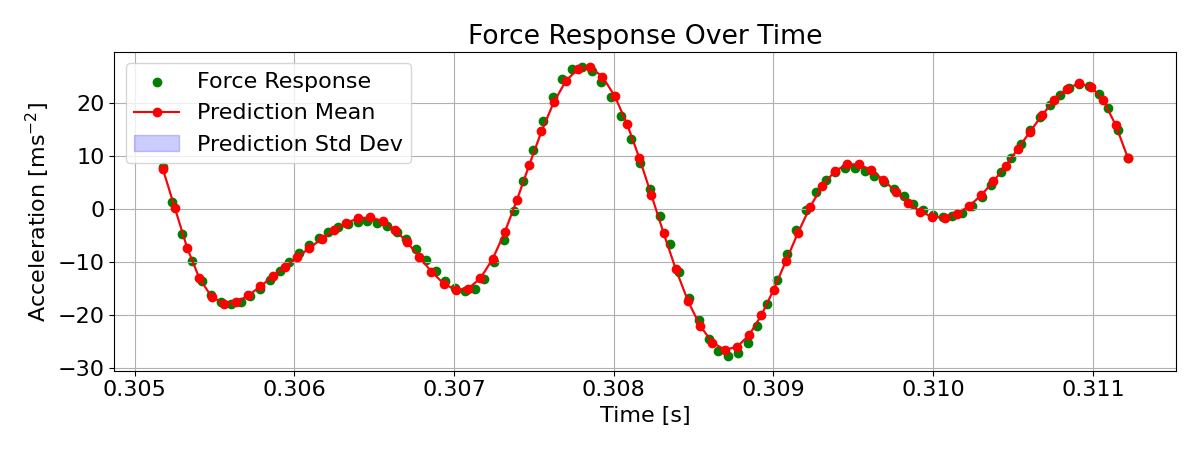
\includegraphics[width=1.0\linewidth]{figures/input-response-plot/input-response-plot.png}
        \caption{The time series data which the GP was fit to.}
        \label{fig:input-response-plot}
    \end{figure}



    \subsection{The Kernel}
    Next, a python class was created to contain the kernel.
    To begin with, a white noise kernel (equation~\ref{eq:white-noise-kernel}) was chosen for the force input plot because there was no trend to the force input data in the centre of the time series data (seconds after the initial impulse from the impact from the hammer).
    This kernel ensures that ``all covariances between samples are zero because the noise is uncorrelated''~\cite{RoelantsGPKernels}

    \begin{equation}
        K_{ij} =
        \begin{cases}
            \sigma^2 & \text{if } \mathbf{x}_i = \mathbf{x}_j \\
            0 & \text{otherwise}
        \end{cases}\label{eq:white-noise-kernel}
    \end{equation}

    For the force response plot, a periodic kernel was chosen (Equation~\ref{eq:periodic-kernel}), which is ideal for such periodic data since it gives pairs of points a high similarity score if the difference between them is near an integer multiple of the `period' hyperparameter.
    The `length' hyperparameter determines how quickly this similarity drops off as the difference between the pair of points changes.
    Practically, this controls how smooth or wiggly the function is, i.e., how fast the function can change direction.

    \begin{equation}
        k(x, x') = \sigma^2 \exp\left(- \frac{2 \sin^2\left(\frac{\pi}{p} |x - x'|\right)}{l^2}\right)\label{eq:periodic-kernel}
    \end{equation}

    \subsection{Hyperparameter Optimisation}
    Next, this kernel class was added as an attribute to a class for the GP model itself.
    This allowed the kernel to be computed for different pairs of arrays as needed.
    This GP model also contained an algorithm to optimise the hyperparameters of the kernel by minimising the Negative Log Marginal Likelihood.
    It did this by multiplying each hyperparameter in turn by the exponent of a normally distributed continuous random variable.
    Imagine that only if the new NLML was lower than the previous, the hyperparameter was updated.
    If this was the case, the algorithm could get stuck in what is known as local minima, and never find the global minimum.
    This would be analogous to a ball always rolling directly downhill to find the global minimum.
    If it got stuck in a small valley half-way down the larger hill, it would never find the lowest point.
    Therefore, a mechanism was added to avoid this:
    If the new NLML was higher than the previous, the hyperparameter was maybe still updated, with a larger probability the closer the NLML was closer to the previous NLML, (i.e., the better the prediction was).

    \subsection{Predict Function}
    Next, the predict function was constructed, which accurately calculated the mean and variance of the output of the latent function when given new test inputs in the continuous input space, as shown in Figure~\ref{fig:input-response-predict}.
    Note that the data is more noisy in the top Force Input than the Force Response plot, so the standard deviation is larger to take account for this noise.

    \begin{figure}[ht]
        \centering
        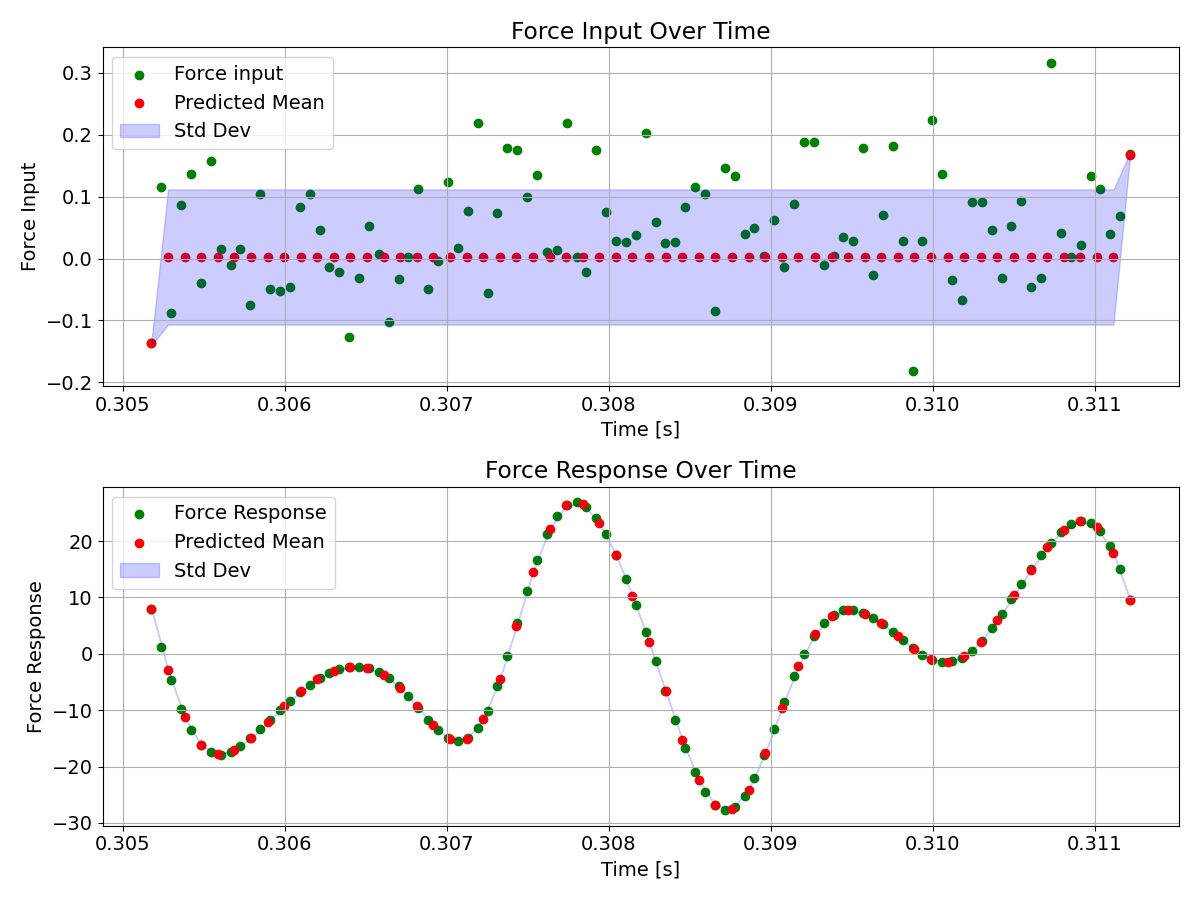
\includegraphics[width=1.0\linewidth]{figures/input-response-predict/input-response-predict.png}
        \caption{The prediction function fit by the GP overlayed on the training data. Note that the standard Deviation increases for data with more noise.}
        \label{fig:input-response-predict}
    \end{figure}

    \subsection{Sparse GP}
    Finally, the model modified to scale to large data, by converting it to a type of Sparse GP approximation known as FITC~\cite{q-candela}.
    This changed the $O()$ from $O(n^3)$ to $O(mn^2)$ for a set of m inducing points chosen to be a subset of the original training points, evenly spaced, where $n \gg m$.
    This modification was made to the NLML and predict functions, which required a very specific implementation involving multiple mathematical tricks in order to keep the calculations numerically stable and efficient in terms of computation time and memory required.
    This is because certain matrix operations such as determinants and inversions can give imprecise results for large matrices containing floating point numbers, which is a format that computers use to store continuous variables as a decimal as opposed to integers type variables.
    After this was complete, the hyperparameters could be optimised and the GP could be fit for functions containing more than 1000 data points in a significantly reduced computation time... %update with times

    \section{Plan for Future Work}
    After the implementation of the Sparse GP, the next step will be to adjust the prediction function for the force input and response plots to be in a closed form.
    This means that the functions will be defined symbolically so that it can be described in general instead of just at a given set of input values, which will allow the closed form Fourier Transform to be taken.
    This can then be solved analytically/symbolically either by hand or using a Python package like SymPy.

    The robustness to noise of the Fourier Transform of this model then needs to be compared to that of the standard discrete Fast Fourier Transform (Objective~\ref{noise-resiliance}).
    To do this, the Frequency Response Function can be computed for both methods by dividing the Fourier Transforms of the force response by that of the force input.
    As a starting point, the Mean Squared Error (MSE) can be computed between the both, to see how different they are.
    The MSE is a method of measuring the quality of an estimator (lower is better) by measuring the average of the squares of the errors, as shown in Equation~\ref{eq:mse}

    \begin{equation}
        \text{MSE} = \frac{1}{n} \sum_{i=1}^{n} (A_i - B_i)^2
        \label{eq:mse}
    \end{equation}


    Then, some Gaussian noise can be added to the data, and the FRF can again be computed using both methods again.
    To find how much each method is corrupted by noise, the (discrete) Mean Squared Error can be computed between the unmodified and noisy FRF for both methods, and the values compared.
    To find how much each method is corrupted by noise, the (discrete) Mean Squared Error can be computed between the unmodified and noisy FRF for both methods, and the values compared.
    Note that for our new closed form Fourier Transform method, it would be possible to use a continuous method to compare the FRF with and without noise.

    If time allows, the stretch objective (\ref{stretch-obj}) of comparing how smoothed out sharp resonance peaks are due to spectral leakage can be complete.
    To do this, the Fourier Transform of a pure sine wave should be found using both the GP and FFT methods.
    This is because it can be solved analytically on paper to provide a Fourier Transform with a sharp peak at the frequency of the wave, and the MSE of each method against the mathematically precise analytical solution can be compared.

    Finally, a conclusion can be drawn regarding the utility of the new Gaussian Process (GP) method of computing the Fourier Transform presented in this paper when compared to the classical Fast Fourier Transform (FFT) with respect to robustness to noise and prevention of artifacts due to spectral leakage.

    \subsection{Future Work Time Plan}
    Figure~\ref{fig:gantt-chart_}a Gantt chart outlining the main steps and the approximate schedule for the remaining work in the project.
    This includes scheduled delays in the Christmas and Easter holidays to allow for exam revision and as a buffer to catch up to the schedule if the project is falling behind:

    \begin{landscape}
        \begin{figure}[p] % 'p' places the figure on a page of its own
            \centering
            \includegraphics[width=\linewidth]{figures/gantt_chart/gantt-chart_.png}
            \caption{A Gantt chart showing work remaining, using a format modified from~\cite{DataCampGanttChart2021}.}
            \label{fig:gantt-chart_}
        \end{figure}
    \end{landscape}

%    \appendix
\section{The use of generative AI (ChatGPT)}
OpenAI's ChatGPT interface, powered by the GPT-4 large language model, was used to implement the Negative Log Marginal Likelihood (NLML) method in my code in a specific way to ensure numerical stability though the use of the ``Cholesky decomposition''.
The prompt and output is provided in Figure~\ref{fig:chat-NLML}.
\begin{figure}[htbp]
    \centering
    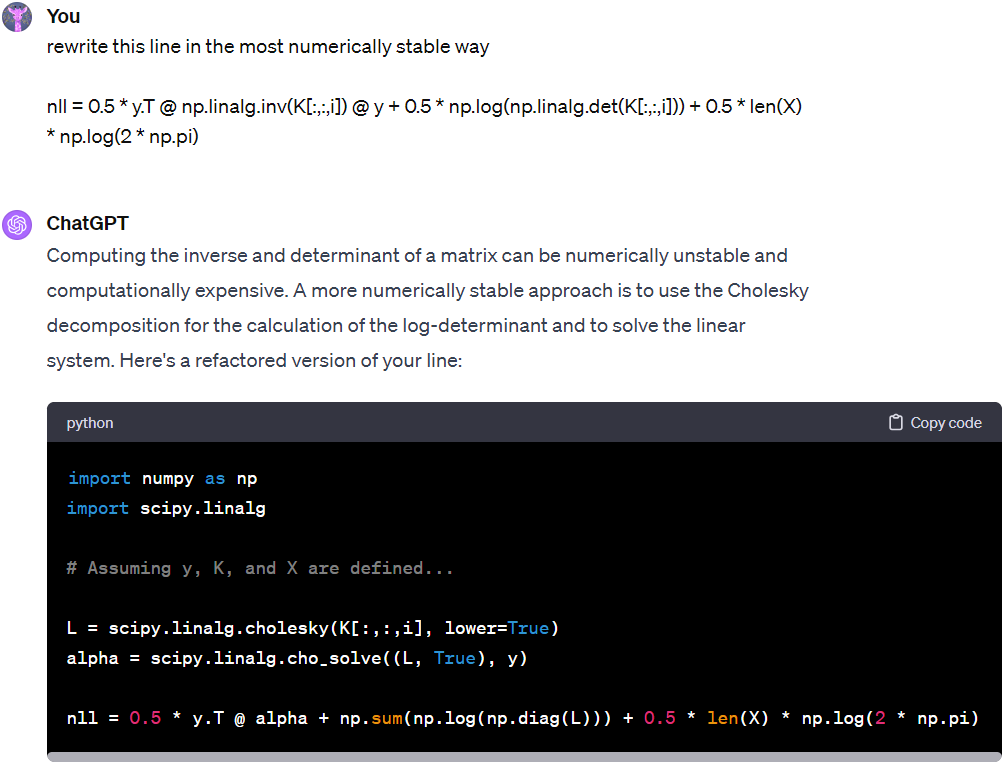
\includegraphics[width=1\linewidth]{figures/chat-NLML/chat-NLML.png}
    \caption{ChatGPT prompt and output providing a way to compute the NLML that is faster and more numerically stable}
    \label{fig:chat-NLML}
\end{figure}

\FloatBarrier

In order to ensure that this function was valid, its implementation was confirmed by the relevant literature~\cite{murphy2023probabilistic}~(Section 18.3.6).
After which, this function was simplified and adapted into that it could be to be added to the $gp\_model$ class as a method, and so that it would work with the way the input data was formatted, as shown in Listing~\ref{1st:NLML}

\begin{lstlisting}[caption={Method used to calculate the Negative Log Marginal Likelihood (NLML).} language=Python,label={lst:NLML}]
    def compute_nlml(self, hyperparameters):
    self.update_hyperparameters_and_debug(hyperparameters)
    self.reshape_X_and_y()

    if self.gp_algo == 'cholesky':
        K = self.gp_kernel.compute_kernel(self.X, self.X)
        K += np.repeat(np.array(np.eye(len(self.X)) * 1e-3)[:,:, np.newaxis], self.X.shape[1], axis=2)
        debug_K = np.squeeze(K)
        L = scipy.linalg.cholesky(K[:, :, 0], lower=True)
        n = len(self.y)
        one_vector = np.ones(n)
        y_adj = self.y - self.y_mean

        alpha = scipy.linalg.cho_solve((L, True), y_adj)

        term_1_c = (0.5 * y_adj.T @ alpha).item()
        term_2_c = np.sum(np.log(np.diag(L)))
        term_3_c = 0.5 * n * np.log(2 * np.pi)

        nlml = term_1_c + term_2_c + term_3_c

        out_c = {
            'nlml': nlml,
            'term_1': term_1_c,
            'term_2': term_2_c,
            'term_3': term_3_c
        }

        return out_c

\end{lstlisting}




    \printbibliography

\end{document}